% Options for packages loaded elsewhere
\PassOptionsToPackage{unicode}{hyperref}
\PassOptionsToPackage{hyphens}{url}
%
\documentclass[
]{book}
\usepackage{lmodern}
\usepackage{amssymb,amsmath}
\usepackage{ifxetex,ifluatex}
\ifnum 0\ifxetex 1\fi\ifluatex 1\fi=0 % if pdftex
  \usepackage[T1]{fontenc}
  \usepackage[utf8]{inputenc}
  \usepackage{textcomp} % provide euro and other symbols
\else % if luatex or xetex
  \usepackage{unicode-math}
  \defaultfontfeatures{Scale=MatchLowercase}
  \defaultfontfeatures[\rmfamily]{Ligatures=TeX,Scale=1}
\fi
% Use upquote if available, for straight quotes in verbatim environments
\IfFileExists{upquote.sty}{\usepackage{upquote}}{}
\IfFileExists{microtype.sty}{% use microtype if available
  \usepackage[]{microtype}
  \UseMicrotypeSet[protrusion]{basicmath} % disable protrusion for tt fonts
}{}
\makeatletter
\@ifundefined{KOMAClassName}{% if non-KOMA class
  \IfFileExists{parskip.sty}{%
    \usepackage{parskip}
  }{% else
    \setlength{\parindent}{0pt}
    \setlength{\parskip}{6pt plus 2pt minus 1pt}}
}{% if KOMA class
  \KOMAoptions{parskip=half}}
\makeatother
\usepackage{xcolor}
\IfFileExists{xurl.sty}{\usepackage{xurl}}{} % add URL line breaks if available
\IfFileExists{bookmark.sty}{\usepackage{bookmark}}{\usepackage{hyperref}}
\hypersetup{
  pdftitle={From Scratch},
  pdfauthor={Patrick Altmeyer},
  hidelinks,
  pdfcreator={LaTeX via pandoc}}
\urlstyle{same} % disable monospaced font for URLs
\usepackage{color}
\usepackage{fancyvrb}
\newcommand{\VerbBar}{|}
\newcommand{\VERB}{\Verb[commandchars=\\\{\}]}
\DefineVerbatimEnvironment{Highlighting}{Verbatim}{commandchars=\\\{\}}
% Add ',fontsize=\small' for more characters per line
\usepackage{framed}
\definecolor{shadecolor}{RGB}{248,248,248}
\newenvironment{Shaded}{\begin{snugshade}}{\end{snugshade}}
\newcommand{\AlertTok}[1]{\textcolor[rgb]{0.94,0.16,0.16}{#1}}
\newcommand{\AnnotationTok}[1]{\textcolor[rgb]{0.56,0.35,0.01}{\textbf{\textit{#1}}}}
\newcommand{\AttributeTok}[1]{\textcolor[rgb]{0.77,0.63,0.00}{#1}}
\newcommand{\BaseNTok}[1]{\textcolor[rgb]{0.00,0.00,0.81}{#1}}
\newcommand{\BuiltInTok}[1]{#1}
\newcommand{\CharTok}[1]{\textcolor[rgb]{0.31,0.60,0.02}{#1}}
\newcommand{\CommentTok}[1]{\textcolor[rgb]{0.56,0.35,0.01}{\textit{#1}}}
\newcommand{\CommentVarTok}[1]{\textcolor[rgb]{0.56,0.35,0.01}{\textbf{\textit{#1}}}}
\newcommand{\ConstantTok}[1]{\textcolor[rgb]{0.00,0.00,0.00}{#1}}
\newcommand{\ControlFlowTok}[1]{\textcolor[rgb]{0.13,0.29,0.53}{\textbf{#1}}}
\newcommand{\DataTypeTok}[1]{\textcolor[rgb]{0.13,0.29,0.53}{#1}}
\newcommand{\DecValTok}[1]{\textcolor[rgb]{0.00,0.00,0.81}{#1}}
\newcommand{\DocumentationTok}[1]{\textcolor[rgb]{0.56,0.35,0.01}{\textbf{\textit{#1}}}}
\newcommand{\ErrorTok}[1]{\textcolor[rgb]{0.64,0.00,0.00}{\textbf{#1}}}
\newcommand{\ExtensionTok}[1]{#1}
\newcommand{\FloatTok}[1]{\textcolor[rgb]{0.00,0.00,0.81}{#1}}
\newcommand{\FunctionTok}[1]{\textcolor[rgb]{0.00,0.00,0.00}{#1}}
\newcommand{\ImportTok}[1]{#1}
\newcommand{\InformationTok}[1]{\textcolor[rgb]{0.56,0.35,0.01}{\textbf{\textit{#1}}}}
\newcommand{\KeywordTok}[1]{\textcolor[rgb]{0.13,0.29,0.53}{\textbf{#1}}}
\newcommand{\NormalTok}[1]{#1}
\newcommand{\OperatorTok}[1]{\textcolor[rgb]{0.81,0.36,0.00}{\textbf{#1}}}
\newcommand{\OtherTok}[1]{\textcolor[rgb]{0.56,0.35,0.01}{#1}}
\newcommand{\PreprocessorTok}[1]{\textcolor[rgb]{0.56,0.35,0.01}{\textit{#1}}}
\newcommand{\RegionMarkerTok}[1]{#1}
\newcommand{\SpecialCharTok}[1]{\textcolor[rgb]{0.00,0.00,0.00}{#1}}
\newcommand{\SpecialStringTok}[1]{\textcolor[rgb]{0.31,0.60,0.02}{#1}}
\newcommand{\StringTok}[1]{\textcolor[rgb]{0.31,0.60,0.02}{#1}}
\newcommand{\VariableTok}[1]{\textcolor[rgb]{0.00,0.00,0.00}{#1}}
\newcommand{\VerbatimStringTok}[1]{\textcolor[rgb]{0.31,0.60,0.02}{#1}}
\newcommand{\WarningTok}[1]{\textcolor[rgb]{0.56,0.35,0.01}{\textbf{\textit{#1}}}}
\usepackage{longtable,booktabs}
% Correct order of tables after \paragraph or \subparagraph
\usepackage{etoolbox}
\makeatletter
\patchcmd\longtable{\par}{\if@noskipsec\mbox{}\fi\par}{}{}
\makeatother
% Allow footnotes in longtable head/foot
\IfFileExists{footnotehyper.sty}{\usepackage{footnotehyper}}{\usepackage{footnote}}
\makesavenoteenv{longtable}
\usepackage{graphicx,grffile}
\makeatletter
\def\maxwidth{\ifdim\Gin@nat@width>\linewidth\linewidth\else\Gin@nat@width\fi}
\def\maxheight{\ifdim\Gin@nat@height>\textheight\textheight\else\Gin@nat@height\fi}
\makeatother
% Scale images if necessary, so that they will not overflow the page
% margins by default, and it is still possible to overwrite the defaults
% using explicit options in \includegraphics[width, height, ...]{}
\setkeys{Gin}{width=\maxwidth,height=\maxheight,keepaspectratio}
% Set default figure placement to htbp
\makeatletter
\def\fps@figure{htbp}
\makeatother
\setlength{\emergencystretch}{3em} % prevent overfull lines
\providecommand{\tightlist}{%
  \setlength{\itemsep}{0pt}\setlength{\parskip}{0pt}}
\setcounter{secnumdepth}{5}
\usepackage{booktabs}
\usepackage{amsthm}
\makeatletter
\def\thm@space@setup{%
  \thm@preskip=8pt plus 2pt minus 4pt
  \thm@postskip=\thm@preskip
}
\makeatother
\usepackage[]{natbib}
\bibliographystyle{apalike}

\title{From Scratch}
\author{Patrick Altmeyer}
\date{2020-10-13}

\begin{document}
\maketitle

{
\setcounter{tocdepth}{1}
\tableofcontents
}
\hypertarget{intro}{%
\chapter{Introduction}\label{intro}}

Introduction

\hypertarget{some-stuff}{%
\section{Some stuff}\label{some-stuff}}

\hypertarget{det-opt}{%
\chapter{Deterministic optimization}\label{det-opt}}

\hypertarget{line-search}{%
\section{Line search}\label{line-search}}

\hypertarget{methodology}{%
\subsection{Methodology}\label{methodology}}

The goal of Exercise 3.1 in \citet{nw2006numerical} is to minimize the bivariate Rosenbrock function (Equation \eqref{eq:rosenbrock}) using \emph{steepest descent} and \emph{Newton's method}. The Rosenbrock function - also known as \emph{Rosenbrock's banana function} - has a long, narrow, parabolic shaped flat valley and is often used for to test optimization algorithms for their performance (see \href{https://en.wikipedia.org/wiki/Rosenbrock_function}{here}).

\begin{equation} 
  f\left(k\right) = \binom{n}{k} p^k\left(1-p\right)^{n-k}
  \label{eq:binom}
\end{equation}

We can implement Equation \eqref{eq:rosenbrock} in R as follows:

\begin{Shaded}
\begin{Highlighting}[]
\CommentTok{# Rosenbrock:}
\NormalTok{f =}\StringTok{ }\ControlFlowTok{function}\NormalTok{(X) \{}
  \DecValTok{100} \OperatorTok{*}\StringTok{ }\NormalTok{(X[}\DecValTok{2}\NormalTok{] }\OperatorTok{-}\StringTok{ }\NormalTok{X[}\DecValTok{1}\NormalTok{]}\OperatorTok{^}\DecValTok{2}\NormalTok{)}\OperatorTok{^}\DecValTok{2} \OperatorTok{+}\StringTok{ }\NormalTok{(}\DecValTok{1} \OperatorTok{-}\StringTok{ }\NormalTok{X[}\DecValTok{1}\NormalTok{])}\OperatorTok{^}\DecValTok{2}
\NormalTok{\}}
\end{Highlighting}
\end{Shaded}

Figure \ref{fig:rosenbrock} shows the output of the function over \(x_1,x_2 \in [-1.5, 1.5]\) along with its minimum indicated as a red asterisk and the two starting points: (1) \(X_0=(1.2,1.2)\) and (2) \(X_0=(-1.2,1)\).

\begin{Shaded}
\begin{Highlighting}[]
\KeywordTok{library}\NormalTok{(ggplot2)}
\CommentTok{# Plot}
\NormalTok{grid =}\StringTok{ }\KeywordTok{data.table}\NormalTok{(}\KeywordTok{expand.grid}\NormalTok{(}\DataTypeTok{x1=}\NormalTok{X_range,}\DataTypeTok{x2=}\NormalTok{X_range))}
\NormalTok{grid[,y}\OperatorTok{:}\ErrorTok{=}\KeywordTok{f}\NormalTok{(}\KeywordTok{c}\NormalTok{(x1,x2)),by=.(}\DecValTok{1}\OperatorTok{:}\KeywordTok{nrow}\NormalTok{(grid))]}
\NormalTok{X_min =}\StringTok{ }\NormalTok{grid[y}\OperatorTok{==}\KeywordTok{min}\NormalTok{(y),.(x1,x2)]}
\NormalTok{p =}\StringTok{ }\KeywordTok{ggplot}\NormalTok{() }\OperatorTok{+}
\StringTok{  }\KeywordTok{geom_contour_filled}\NormalTok{(}\DataTypeTok{data =}\NormalTok{ grid, }\KeywordTok{aes}\NormalTok{(}\DataTypeTok{x=}\NormalTok{x1,}\DataTypeTok{y=}\NormalTok{x2,}\DataTypeTok{z=}\NormalTok{y)) }\OperatorTok{+}
\StringTok{  }\KeywordTok{geom_point}\NormalTok{(}\DataTypeTok{data =}\NormalTok{ X_min, }\KeywordTok{aes}\NormalTok{(}\DataTypeTok{x=}\NormalTok{x1,}\DataTypeTok{y=}\NormalTok{x2), }\DataTypeTok{colour=}\StringTok{"red"}\NormalTok{, }\DataTypeTok{shape=}\DecValTok{8}\NormalTok{) }\OperatorTok{+}
\StringTok{  }\KeywordTok{geom_point}\NormalTok{(}\DataTypeTok{data =}\NormalTok{ X0, }\KeywordTok{aes}\NormalTok{(}\DataTypeTok{x=}\NormalTok{x1,}\DataTypeTok{y=}\NormalTok{x2), }\DataTypeTok{colour=}\StringTok{"red"}\NormalTok{) }\OperatorTok{+}\StringTok{ }
\StringTok{  }\KeywordTok{geom_text}\NormalTok{(}\DataTypeTok{data =}\NormalTok{ X0, }\KeywordTok{aes}\NormalTok{(}\DataTypeTok{x=}\NormalTok{x1,}\DataTypeTok{y=}\NormalTok{x2,}\DataTypeTok{label=}\NormalTok{label), }\DataTypeTok{colour=}\StringTok{"red"}\NormalTok{, }\DataTypeTok{nudge_x =} \FloatTok{0.1}\NormalTok{, }\DataTypeTok{nudge_y =} \FloatTok{0.1}\NormalTok{)}
\NormalTok{p}
\end{Highlighting}
\end{Shaded}

\begin{figure}
\centering
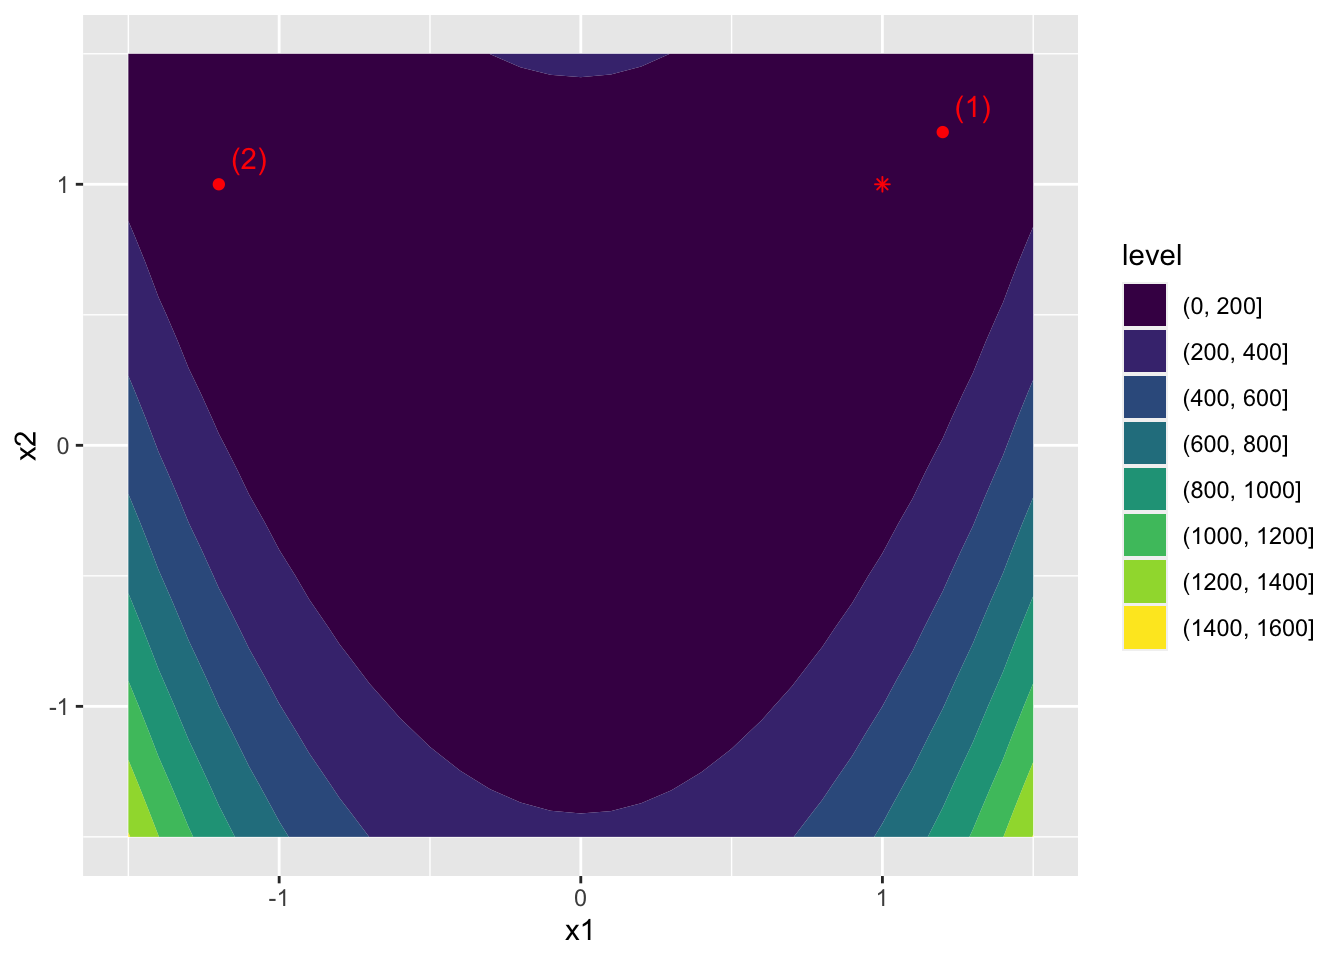
\includegraphics{fromScratch_files/figure-latex/rosenbrock-1.pdf}
\caption{\label{fig:rosenbrock}Output of the Rosenbrock function and minimizer in red.}
\end{figure}

The gradient and Hessian of \(f\) can be computed as

and

which in R can be encoded as follows:

\begin{Shaded}
\begin{Highlighting}[]
\CommentTok{# Gradient:}
\NormalTok{df =}\StringTok{ }\ControlFlowTok{function}\NormalTok{(X) \{}
\NormalTok{  df =}\StringTok{ }\KeywordTok{rep}\NormalTok{(}\DecValTok{0}\NormalTok{, }\KeywordTok{length}\NormalTok{(X))}
\NormalTok{  df[}\DecValTok{1}\NormalTok{] =}\StringTok{ }\DecValTok{-400} \OperatorTok{*}\StringTok{ }\NormalTok{X[}\DecValTok{1}\NormalTok{]}\OperatorTok{^}\DecValTok{2} \OperatorTok{*}\StringTok{ }\NormalTok{(X[}\DecValTok{2}\NormalTok{] }\OperatorTok{-}\StringTok{ }\NormalTok{X[}\DecValTok{1}\NormalTok{]}\OperatorTok{^}\DecValTok{2}\NormalTok{) }\OperatorTok{-}\StringTok{ }\DecValTok{2} \OperatorTok{*}\StringTok{ }\NormalTok{(}\DecValTok{1} \OperatorTok{-}\StringTok{ }\NormalTok{X[}\DecValTok{1}\NormalTok{]) }\CommentTok{# partial with respect to x_1}
\NormalTok{  df[}\DecValTok{2}\NormalTok{] =}\StringTok{ }\DecValTok{200} \OperatorTok{*}\StringTok{ }\NormalTok{(X[}\DecValTok{2}\NormalTok{] }\OperatorTok{-}\StringTok{ }\NormalTok{X[}\DecValTok{1}\NormalTok{]}\OperatorTok{^}\DecValTok{2}\NormalTok{)}
  \KeywordTok{return}\NormalTok{(df)}
\NormalTok{\}}

\CommentTok{# Hessian:}
\NormalTok{ddf =}\StringTok{ }\ControlFlowTok{function}\NormalTok{(X) \{}
\NormalTok{  ddf =}\StringTok{ }\KeywordTok{matrix}\NormalTok{(}\DataTypeTok{nrow =} \KeywordTok{length}\NormalTok{(X), }\DataTypeTok{ncol=}\KeywordTok{length}\NormalTok{(X))}
\NormalTok{  ddf[}\DecValTok{1}\NormalTok{,}\DecValTok{1}\NormalTok{] =}\StringTok{ }\DecValTok{1200} \OperatorTok{*}\StringTok{ }\NormalTok{X[}\DecValTok{1}\NormalTok{]}\OperatorTok{^}\DecValTok{2} \OperatorTok{-}\StringTok{ }\DecValTok{400} \OperatorTok{*}\StringTok{ }\NormalTok{X[}\DecValTok{2}\NormalTok{] }\OperatorTok{+}\StringTok{ }\DecValTok{2} \CommentTok{# partial with respect to x_1}
\NormalTok{  ddf[}\DecValTok{2}\NormalTok{,}\DecValTok{1}\NormalTok{] =}\StringTok{ }\NormalTok{ddf[}\DecValTok{1}\NormalTok{,}\DecValTok{2}\NormalTok{] =}\StringTok{ }\DecValTok{-400} \OperatorTok{*}\StringTok{ }\NormalTok{X[}\DecValTok{1}\NormalTok{]}
\NormalTok{  ddf[}\DecValTok{2}\NormalTok{,}\DecValTok{2}\NormalTok{] =}\StringTok{ }\DecValTok{200}
  \KeywordTok{return}\NormalTok{(ddf)}
\NormalTok{\}}
\end{Highlighting}
\end{Shaded}

For both methods I will use the \emph{Arminjo condition} with backtracking. The \texttt{gradient\_desc} function (below) can implement both \emph{steepest descent} and \emph{Newton's method}. The code for the function can be inspected below (you can reveal it by simply clicking on the \emph{Code} button on the right). There's also a small description of the different arguments.

\begin{Shaded}
\begin{Highlighting}[]
\CommentTok{#' Gradient descent}
\CommentTok{#'}
\CommentTok{#' @param f Function to be optimized.}
\CommentTok{#' @param df Gradient of function.}
\CommentTok{#' @param c Constant used in backtrack condition.}
\CommentTok{#' @param method Descent method.}
\CommentTok{#' @param X0 Initial guess.}
\CommentTok{#' @param step_size0 Initial step size.}
\CommentTok{#' @param ddf Hessian.}
\CommentTok{#' @param remember Boolean: should points visited and steps be stored?}
\CommentTok{#' @param tau Parameter governing the tolerance for convergence.}
\CommentTok{#' @param backtrack_cond Backtrack method.}
\CommentTok{#' @param max_iter Maximum number of iterations.}
\CommentTok{#'}
\CommentTok{#' @return}
\CommentTok{#' @export}
\CommentTok{#'}
\CommentTok{#' @examples}
\NormalTok{gradient_desc =}\StringTok{ }\ControlFlowTok{function}\NormalTok{(}
\NormalTok{  f,df,X0,}
  \DataTypeTok{step_size0=}\DecValTok{1}\NormalTok{,}
  \DataTypeTok{ddf=}\OtherTok{NULL}\NormalTok{,}
  \DataTypeTok{method=}\StringTok{"newton"}\NormalTok{,}
  \DataTypeTok{c=}\FloatTok{1e-4}\NormalTok{,}
  \DataTypeTok{remember=}\OtherTok{TRUE}\NormalTok{,}
  \DataTypeTok{tau=}\FloatTok{1e-5}\NormalTok{,}
  \DataTypeTok{backtrack_cond =} \StringTok{"arminjo"}\NormalTok{,}
  \DataTypeTok{max_iter=}\DecValTok{10000}
\NormalTok{) \{}
  \CommentTok{# Initialization: ----}
\NormalTok{  X_latest =}\StringTok{ }\KeywordTok{matrix}\NormalTok{(X0)}
  \ControlFlowTok{if}\NormalTok{ (remember) \{}
\NormalTok{    X =}\StringTok{ }\KeywordTok{matrix}\NormalTok{(X0,}\DataTypeTok{ncol=}\KeywordTok{length}\NormalTok{(X0))}
\NormalTok{    steps =}\StringTok{ }\KeywordTok{matrix}\NormalTok{(}\DataTypeTok{ncol=}\KeywordTok{length}\NormalTok{(X0))}
\NormalTok{  \}}
\NormalTok{  iter =}\StringTok{ }\DecValTok{0}
  \CommentTok{# Set-up based on method:}
  \ControlFlowTok{if}\NormalTok{ (method}\OperatorTok{==}\StringTok{"steepest"}\NormalTok{) \{}
\NormalTok{    B =}\StringTok{ }\ControlFlowTok{function}\NormalTok{(X) \{}
      \KeywordTok{diag}\NormalTok{(}\KeywordTok{length}\NormalTok{(X)) }\CommentTok{# identity}
\NormalTok{    \}}
\NormalTok{  \} }\ControlFlowTok{else} \ControlFlowTok{if}\NormalTok{ (method}\OperatorTok{==}\StringTok{"newton"}\NormalTok{) \{}
\NormalTok{    B =}\StringTok{ }\KeywordTok{tryCatch}\NormalTok{(ddf, }\DataTypeTok{error=}\ControlFlowTok{function}\NormalTok{(e) \{}
      \KeywordTok{stop}\NormalTok{(}\StringTok{"Hessian needs to be supplied for Newton's method."}\NormalTok{)}
\NormalTok{    \}) }\CommentTok{# Hessian}
\NormalTok{  \}}
  \CommentTok{# Backtrack condition}
  \ControlFlowTok{if}\NormalTok{ (backtrack_cond}\OperatorTok{==}\StringTok{"arminjo"}\NormalTok{) \{}
\NormalTok{    sufficient_decrease =}\StringTok{ }\ControlFlowTok{function}\NormalTok{(alpha) \{}
      \KeywordTok{return}\NormalTok{(}\KeywordTok{f}\NormalTok{(X_k }\OperatorTok{+}\StringTok{ }\NormalTok{alpha }\OperatorTok{*}\StringTok{ }\NormalTok{p_k) }\OperatorTok{<=}\StringTok{ }\KeywordTok{f}\NormalTok{(X_k) }\OperatorTok{+}\StringTok{ }\NormalTok{c }\OperatorTok{*}\StringTok{ }\NormalTok{alpha }\OperatorTok{*}\StringTok{ }\KeywordTok{t}\NormalTok{(df_k) }\OperatorTok\StringTok{ }\NormalTok{p_k) }\CommentTok{# Arminjo condition}
\NormalTok{    \}}
\NormalTok{  \} }\ControlFlowTok{else} \ControlFlowTok{if}\NormalTok{ (}\KeywordTok{is.na}\NormalTok{(backtrack_cond)) \{}
\NormalTok{    sufficient_decrease =}\StringTok{ }\ControlFlowTok{function}\NormalTok{(alpha) \{}
      \KeywordTok{return}\NormalTok{(}\KeywordTok{f}\NormalTok{(X_k }\OperatorTok{+}\StringTok{ }\NormalTok{alpha }\OperatorTok{*}\StringTok{ }\NormalTok{p_k) }\OperatorTok{<=}\StringTok{ }\KeywordTok{f}\NormalTok{(X_k)) }\CommentTok{# Standard condition}
\NormalTok{    \}}
\NormalTok{  \}}
  \CommentTok{# Run algorithm: ----}
  \ControlFlowTok{while}\NormalTok{ (}\KeywordTok{any}\NormalTok{(}\KeywordTok{abs}\NormalTok{(}\KeywordTok{df}\NormalTok{(X_latest)}\OperatorTok{-}\KeywordTok{rep}\NormalTok{(}\DecValTok{0}\NormalTok{,}\KeywordTok{length}\NormalTok{(X_latest)))}\OperatorTok{>}\NormalTok{tau) }\OperatorTok{&}\StringTok{ }\NormalTok{iter }\OperatorTok{<}\StringTok{ }\NormalTok{max_iter) \{ }\CommentTok{# first-order condition}
\NormalTok{    X_k =}\StringTok{ }\NormalTok{X_latest}
\NormalTok{    alpha =}\StringTok{ }\NormalTok{step_size0 }\CommentTok{# initialize step size}
\NormalTok{    df_k =}\StringTok{ }\KeywordTok{matrix}\NormalTok{(}\KeywordTok{df}\NormalTok{(X_latest))}
\NormalTok{    B_k =}\StringTok{ }\KeywordTok{B}\NormalTok{(X_latest)}
\NormalTok{    p_k =}\StringTok{ }\OperatorTok{-}\StringTok{ }\NormalTok{(}\KeywordTok{solve}\NormalTok{(B_k) }\OperatorTok\StringTok{ }\NormalTok{df_k)}
    \CommentTok{# Backtracking:}
    \ControlFlowTok{while}\NormalTok{ (}\OperatorTok{!}\KeywordTok{sufficient_decrease}\NormalTok{(alpha)) \{}
\NormalTok{      alpha =}\StringTok{ }\NormalTok{alpha}\OperatorTok{/}\DecValTok{2}
\NormalTok{    \}}
    \CommentTok{# Update:}
\NormalTok{    X_latest =}\StringTok{ }\NormalTok{X_latest }\OperatorTok{+}\StringTok{ }\NormalTok{alpha }\OperatorTok{*}\StringTok{ }\NormalTok{p_k}
\NormalTok{    iter =}\StringTok{ }\NormalTok{iter }\OperatorTok{+}\StringTok{ }\DecValTok{1}
    \ControlFlowTok{if}\NormalTok{ (remember) \{}
\NormalTok{      X =}\StringTok{ }\KeywordTok{rbind}\NormalTok{(X, }\KeywordTok{t}\NormalTok{(X_latest))}
\NormalTok{      steps =}\StringTok{ }\KeywordTok{rbind}\NormalTok{(steps, }\KeywordTok{t}\NormalTok{(alpha }\OperatorTok{*}\StringTok{ }\NormalTok{p_k))}
\NormalTok{    \}}
\NormalTok{  \}}
  \ControlFlowTok{if}\NormalTok{ (iter}\OperatorTok{>=}\NormalTok{max_iter) }\KeywordTok{warning}\NormalTok{(}\StringTok{"Reached maximum number of iterations without convergence."}\NormalTok{)}
  \CommentTok{# Tidy up: ----}
\NormalTok{  output =}\StringTok{ }\KeywordTok{list}\NormalTok{(}
    \DataTypeTok{optimal =}\NormalTok{ X_latest,}
    \DataTypeTok{visited =} \KeywordTok{tryCatch}\NormalTok{(X, }\DataTypeTok{error=}\ControlFlowTok{function}\NormalTok{(e) }\OtherTok{NULL}\NormalTok{),}
    \DataTypeTok{steps =} \KeywordTok{tryCatch}\NormalTok{(steps, }\DataTypeTok{error=}\ControlFlowTok{function}\NormalTok{(e) }\OtherTok{NULL}\NormalTok{),}
    \DataTypeTok{X0 =}\NormalTok{ X0,}
    \DataTypeTok{method =}\NormalTok{ method}
\NormalTok{  )}
  \KeywordTok{return}\NormalTok{(output)}
\NormalTok{\}}
\end{Highlighting}
\end{Shaded}

Similarly you can take a look at how the \texttt{gradient\_desc} is applied in the underlying problem by unhiding the next code chunk.

\begin{Shaded}
\begin{Highlighting}[]
\KeywordTok{source}\NormalTok{(}\StringTok{"R/gradient_desc.R"}\NormalTok{)}
\NormalTok{init_guesses =}\StringTok{ }\DecValTok{1}\OperatorTok{:}\KeywordTok{nrow}\NormalTok{(X0)}
\NormalTok{algos =}\StringTok{ }\KeywordTok{c}\NormalTok{(}\StringTok{"steepest"}\NormalTok{,}\StringTok{"newton"}\NormalTok{)}
\NormalTok{grid =}\StringTok{ }\KeywordTok{expand.grid}\NormalTok{(}\DataTypeTok{guess=}\NormalTok{init_guesses,}\DataTypeTok{algo=}\NormalTok{algos)}
\NormalTok{X_star =}\StringTok{ }\KeywordTok{lapply}\NormalTok{(}
  \DecValTok{1}\OperatorTok{:}\KeywordTok{nrow}\NormalTok{(grid),}
  \ControlFlowTok{function}\NormalTok{(i) \{}
    \KeywordTok{gradient_desc}\NormalTok{(}
      \DataTypeTok{f=}\NormalTok{f,}\DataTypeTok{df=}\NormalTok{df,}
      \DataTypeTok{X0=}\NormalTok{X0[grid[i,}\StringTok{"guess"}\NormalTok{],}\KeywordTok{c}\NormalTok{(x1,x2)],}
      \DataTypeTok{method =}\NormalTok{ grid[i,}\StringTok{"algo"}\NormalTok{]}
\NormalTok{    )}
\NormalTok{  \}}
\NormalTok{)}
\CommentTok{# Tidy up}
\NormalTok{X_star_dt =}\StringTok{ }\KeywordTok{rbindlist}\NormalTok{(}
  \KeywordTok{lapply}\NormalTok{(}
    \DecValTok{1}\OperatorTok{:}\KeywordTok{length}\NormalTok{(X_star), }
    \ControlFlowTok{function}\NormalTok{(i) \{}
\NormalTok{      dt =}\StringTok{ }\KeywordTok{data.table}\NormalTok{(X_star[[i]]}\OperatorTok{$}\NormalTok{visited)}
\NormalTok{      dt[,method}\OperatorTok{:}\ErrorTok{=}\NormalTok{X_star[[i]]}\OperatorTok{$}\NormalTok{method]}
\NormalTok{      dt[,(}\KeywordTok{c}\NormalTok{(}\StringTok{"x0_1"}\NormalTok{,}\StringTok{"x0_2"}\NormalTok{))}\OperatorTok{:}\ErrorTok{=}\NormalTok{.(X_star[[i]]}\OperatorTok{$}\NormalTok{X0[}\DecValTok{1}\NormalTok{],X_star[[i]]}\OperatorTok{$}\NormalTok{X0[}\DecValTok{2}\NormalTok{])]}
\NormalTok{      dt[,iteration}\OperatorTok{:}\ErrorTok{=}\NormalTok{.I}\DecValTok{-1}\NormalTok{]}
\NormalTok{      dt[,y}\OperatorTok{:}\ErrorTok{=}\KeywordTok{f}\NormalTok{(}\KeywordTok{c}\NormalTok{(V1,V2)),by=.(}\DecValTok{1}\OperatorTok{:}\KeywordTok{nrow}\NormalTok{(dt))]}
\NormalTok{    \}}
\NormalTok{  )}
\NormalTok{)}
\end{Highlighting}
\end{Shaded}

\hypertarget{results}{%
\subsection{Results}\label{results}}

The below shows how the two algorithms converge to

\begin{figure}
\centering
\includegraphics{www/p1.gif}
\caption{Good initial guess}
\end{figure}

\begin{figure}
\centering
\includegraphics{www/p2.gif}
\caption{Poor initial guess}
\end{figure}

\begin{Shaded}
\begin{Highlighting}[]
\KeywordTok{library}\NormalTok{(gganimate)}
\KeywordTok{library}\NormalTok{(transformr)}
\KeywordTok{library}\NormalTok{(gridExtra)}
\NormalTok{chart_dt =}\StringTok{ }\NormalTok{X_star_dt[x0_}\DecValTok{1}\OperatorTok{==}\NormalTok{X0[}\DecValTok{1}\NormalTok{,x1] }\OperatorTok{&}\StringTok{ }\NormalTok{x0_}\DecValTok{2}\OperatorTok{==}\NormalTok{X0[}\DecValTok{1}\NormalTok{,x2]]}
\CommentTok{# Data for descent path:}
\NormalTok{desc_dt =}\StringTok{ }\NormalTok{chart_dt[,keep}\OperatorTok{:}\ErrorTok{=}\NormalTok{iteration}\OperatorTok\NormalTok{iteration[}\KeywordTok{unique}\NormalTok{(}\KeywordTok{floor}\NormalTok{(}\KeywordTok{seq}\NormalTok{(}\DecValTok{1}\NormalTok{, .N, }\DataTypeTok{length.out =} \DecValTok{10}\NormalTok{)))],by=.(method)][keep}\OperatorTok{==}\NormalTok{T][,keep}\OperatorTok{:}\ErrorTok{=}\OtherTok{NULL}\NormalTok{]}
\NormalTok{desc_dt[,state}\OperatorTok{:}\ErrorTok{=}\DecValTok{1}\OperatorTok{:}\NormalTok{.N,by=.(method)]}
\CommentTok{# Data for function values (contour plot):}
\NormalTok{X_seq =}\StringTok{ }\NormalTok{desc_dt[,.(}\DataTypeTok{seq=}\NormalTok{\{}
\NormalTok{  X_range =}\StringTok{ }\KeywordTok{range}\NormalTok{(}\KeywordTok{c}\NormalTok{(V1,V2))}
\NormalTok{  X_seq =}\StringTok{ }\KeywordTok{seq}\NormalTok{(X_range[}\DecValTok{1}\NormalTok{],X_range[}\DecValTok{2}\NormalTok{],}\DataTypeTok{length.out =} \DecValTok{10}\NormalTok{)}
\NormalTok{\})]}\OperatorTok{$}\NormalTok{seq}
\NormalTok{contour_dt =}\StringTok{ }\NormalTok{desc_dt[,}\KeywordTok{expand.grid}\NormalTok{(}\DataTypeTok{V1=}\NormalTok{X_seq,}\DataTypeTok{V2=}\NormalTok{X_seq),by=.(method)]}
\NormalTok{contour_dt[,y}\OperatorTok{:}\ErrorTok{=}\KeywordTok{f}\NormalTok{(}\KeywordTok{c}\NormalTok{(V1,V2)),by=.(}\DecValTok{1}\OperatorTok{:}\KeywordTok{nrow}\NormalTok{(contour_dt))]}
\CommentTok{# Data for initial guesses and optimum:}
\NormalTok{start_dt =}\StringTok{ }\KeywordTok{unique}\NormalTok{(chart_dt[,.(method,}\DataTypeTok{x1=}\NormalTok{x0_}\DecValTok{1}\NormalTok{,}\DataTypeTok{x2=}\NormalTok{x0_}\DecValTok{2}\NormalTok{)])}
\NormalTok{start_dt[,which}\OperatorTok{:}\ErrorTok{=}\StringTok{"start"}\NormalTok{]}
\NormalTok{end_dt =}\StringTok{ }\NormalTok{X_min[,.(}\DataTypeTok{method =}\NormalTok{ start_end_dt}\OperatorTok{$}\NormalTok{method, x1, x2,}\DataTypeTok{which=}\StringTok{"end"}\NormalTok{)]}
\NormalTok{start_end_dt =}\StringTok{ }\KeywordTok{rbind}\NormalTok{(start_dt,end_dt)}
\NormalTok{p =}\StringTok{ }\KeywordTok{ggplot}\NormalTok{() }\OperatorTok{+}
\StringTok{  }\CommentTok{# Contour plot:}
\StringTok{  }\KeywordTok{geom_contour}\NormalTok{(}
    \DataTypeTok{data =}\NormalTok{ contour_dt,}
    \KeywordTok{aes}\NormalTok{(}\DataTypeTok{x=}\NormalTok{V1, }\DataTypeTok{y=}\NormalTok{V2, }\DataTypeTok{z=}\NormalTok{y),}
    \DataTypeTok{bins =} \DecValTok{20}
\NormalTok{  ) }\OperatorTok{+}
\StringTok{  }\CommentTok{# Start:}
\StringTok{  }\KeywordTok{geom_point}\NormalTok{(}
    \DataTypeTok{data=}\NormalTok{start_end_dt,}
    \KeywordTok{aes}\NormalTok{(}\DataTypeTok{x=}\NormalTok{x1, }\DataTypeTok{y=}\NormalTok{x2, }\DataTypeTok{shape=}\NormalTok{which),}
    \DataTypeTok{colour=}\StringTok{"red"}
\NormalTok{  ) }\OperatorTok{+}
\StringTok{  }\CommentTok{# Descent path:}
\StringTok{  }\KeywordTok{geom_point}\NormalTok{(}
    \DataTypeTok{data =}\NormalTok{ desc_dt,}
    \KeywordTok{aes}\NormalTok{(}\DataTypeTok{x=}\NormalTok{V1, }\DataTypeTok{y=}\NormalTok{V2),}
    \DataTypeTok{colour=}\StringTok{"black"}\NormalTok{,}
    \DataTypeTok{size=}\FloatTok{0.75}
\NormalTok{  ) }\OperatorTok{+}
\StringTok{  }\CommentTok{# Iteration count:}
\StringTok{  }\KeywordTok{geom_label}\NormalTok{(}
    \DataTypeTok{data =}\NormalTok{ desc_dt,}
    \KeywordTok{aes}\NormalTok{(}\DataTypeTok{x=}\KeywordTok{min}\NormalTok{(X_seq), }\DataTypeTok{y=}\KeywordTok{max}\NormalTok{(X_seq), }\DataTypeTok{label=}\KeywordTok{paste0}\NormalTok{(}\StringTok{"Count: "}\NormalTok{,iteration)),}
    \DataTypeTok{nudge_x=}\KeywordTok{diff}\NormalTok{(}\KeywordTok{range}\NormalTok{(X_seq))}\OperatorTok{*}\FloatTok{0.25}\NormalTok{,}
    \DataTypeTok{nudge_y=}\OperatorTok{-}\KeywordTok{diff}\NormalTok{(}\KeywordTok{range}\NormalTok{(X_seq)}\OperatorTok{*}\FloatTok{0.1}\NormalTok{)}
\NormalTok{  ) }\OperatorTok{+}
\StringTok{  }\CommentTok{# Formatting:}
\StringTok{  }\KeywordTok{scale_y_continuous}\NormalTok{(}
    \DataTypeTok{expand =} \KeywordTok{c}\NormalTok{(}\FloatTok{0.005}\NormalTok{,}\FloatTok{0.005}\NormalTok{)}
\NormalTok{  ) }\OperatorTok{+}
\StringTok{  }\KeywordTok{scale_x_continuous}\NormalTok{(}
    \DataTypeTok{expand =} \KeywordTok{c}\NormalTok{(}\FloatTok{0.005}\NormalTok{,}\FloatTok{0.005}\NormalTok{)}
\NormalTok{  ) }\OperatorTok{+}
\StringTok{  }\KeywordTok{labs}\NormalTok{(}
    \DataTypeTok{x=}\StringTok{"x1"}\NormalTok{,}
    \DataTypeTok{y=}\StringTok{"x2"}
\NormalTok{  ) }\OperatorTok{+}
\StringTok{  }\KeywordTok{scale_shape_manual}\NormalTok{(}
    \DataTypeTok{name=}\StringTok{"Point:"}\NormalTok{,}
    \DataTypeTok{values=}\KeywordTok{c}\NormalTok{(}\DecValTok{8}\NormalTok{,}\DecValTok{19}\NormalTok{)}
\NormalTok{  ) }\OperatorTok{+}
\StringTok{  }\CommentTok{# Facetting:}
\StringTok{  }\KeywordTok{facet_grid}\NormalTok{(}
    \DataTypeTok{cols =} \KeywordTok{vars}\NormalTok{(method)}
\NormalTok{  ) }\OperatorTok{+}
\StringTok{  }\CommentTok{# Animation:}
\StringTok{  }\KeywordTok{transition_states}\NormalTok{(}
\NormalTok{    desc_dt}\OperatorTok{$}\NormalTok{state,}
    \DataTypeTok{transition_length =} \DecValTok{2}\NormalTok{,}
    \DataTypeTok{state_length =} \DecValTok{1}
\NormalTok{  ) }\OperatorTok{+}
\StringTok{  }\KeywordTok{enter_fade}\NormalTok{() }\OperatorTok{+}
\StringTok{  }\KeywordTok{ease_aes}\NormalTok{(}\StringTok{'sine-in-out'}\NormalTok{) }\OperatorTok{+}
\StringTok{  }\KeywordTok{shadow_trail}\NormalTok{(}\DataTypeTok{distance =} \FloatTok{0.05}\NormalTok{)}
\KeywordTok{anim_save}\NormalTok{(}\StringTok{"www/p1.gif"}\NormalTok{,p, }\DataTypeTok{width =} \DecValTok{800}\NormalTok{, }\DataTypeTok{height =} \DecValTok{400}\NormalTok{)}
\end{Highlighting}
\end{Shaded}

\hypertarget{references}{%
\section{References}\label{references}}

  \bibliography{bib.bib,packages.bib}

\end{document}
